\begin{figure}
\centering
\begin{minipage}{1.0\textwidth}    
  \centering
  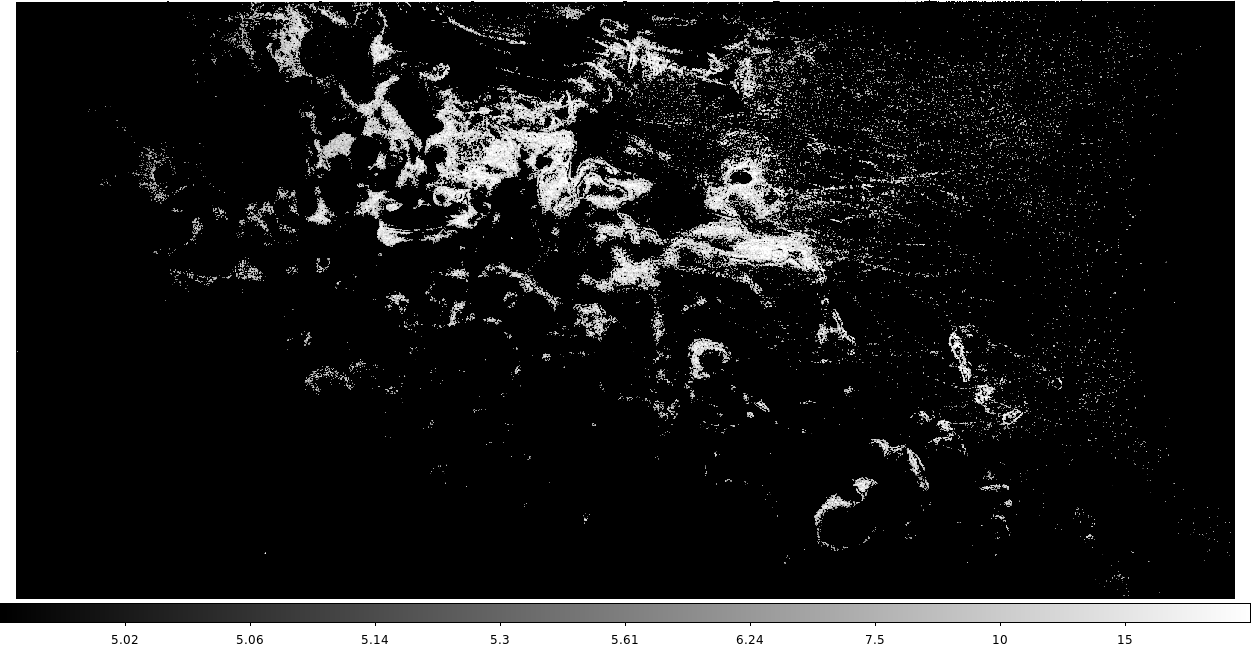
\includegraphics[width=.95\linewidth]{figures/phosphorescence-survey/stains_phos.png}    
\end{minipage}
\begin{minipage}{1.0\textwidth}
  \centering
  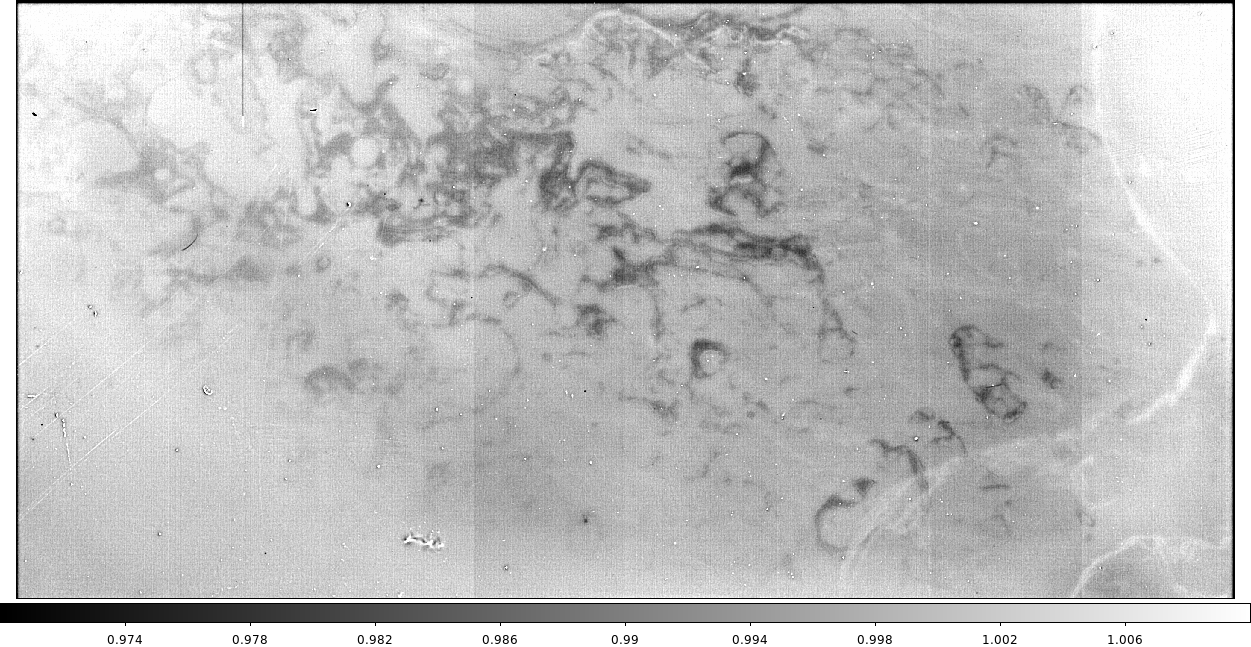
\includegraphics[width=.95\linewidth]{figures/phosphorescence-survey/stains_abs.png}
\end{minipage}
\caption{R00\_SW1 image showing phosphorescence (top) with morphology similar to the ``coffee stains'' (bottom) observed with {\it blue} CCOB LED illumination. The phosphorescence acquired in dark exposures within the first 15\,s following trigger (top) uses a logarithmic stretch with limits 5--25 e$^-$/pixel. The {\it blue} flat field (bottom) is displayed normalized, with 4\% stretch limits (0.97 to 1.01), for a target signal level of $10^4$ e$^-$/pixel. Note that the phosphorescence pattern resembles the dark wisps in the flat (with opposite polarity) but that there are apparently no significant phosphorescence features corresponding to the bright wisps.}
\label{fig:phos:stains}
\end{figure}
